\documentclass[sigplan, screen]{acmart}
\AtBeginDocument{%
  \providecommand\BibTeX{{%
    \normalfont B\kern-0.5em{\scshape i\kern-0.25em b}\kern-0.8em\TeX}}}



\usepackage{subfigure}
\usepackage{caption}
\usepackage{algorithm}
\usepackage{algpseudocode}

\algdef{SE}{Begin}{End}{\textbf{begin}}{\textbf{end}}
\def\BState{\State\hskip-.5em}
%%
%% end of the preamble, start of the body of the document source.
\begin{document}

%%
%% The "title" command has an optional parameter,
%% allowing the author to define a "short title" to be used in page headers.
\title{Generating Trigger-Action Program from Traces\\Based on Association Rule Mining: A Survey}

%%
%% The "author" command and its associated commands are used to define
%% the authors and their affiliations.
%% Of note is the shared affiliation of the first two authors, and the
%% "authornote" and "authornotemark" commands
%% used to denote shared contribution to the research.
\author{Yicheng Wang}
\affiliation{%
  \institution{Institute of Software \\ Chinese Academy of Sciences}
  \city{Haidian Qu}
  \state{Beijing}
  \country{China}
}
\email{wangyicheng215@mails.ucas.ac.cn}

%%
%% By default, the full list of authors will be used in the page
%% headers. Often, this list is too long, and will overlap
%% other information printed in the page headers. This command allows
%% the author to define a more concise list
%% of authors' names for this purpose.
\renewcommand{\shortauthors}{Yicheng Wang}

%%
%% The abstract is a short summary of the work to be presented in the
%% article.
\begin{abstract}
  Trigger-action programming (TAP) is a novel approch to define connections between different Internet of Things (IoT) devices and services,
  which could translate human’s intent of IoT devices into desired automation. User-written TAP rules have been widely used
  as a programming interface in popular IoT systems.
  As users may experience difficulties in discovering related devices functionality and designing rules, recent works try to
  automatically generate TAP rules from past user event traces (time-stamped logs of sensor readings and manual actuations of devices).
  which turns problem into association rule mining of user's trace sequences.

  This survey presents a taxonomy of classic association rule mining (ARM) algorithms, indicates the basic workflow and the important key features of these
  representative algorithms. We also investigate the meritorious applications in Ambient Intelligence (AmI) area, which utilize ARM algorithms to mining the frequent 
  pattern in user event traces, and classify the applications by the algorithms they use. This survey serves as an introduction for IoT related researchers who 
  are intend to realize smart device automation by past behavior mining, and we identifies notable opportunities for further work.


  
\end{abstract}

%%
%% The code below is generated by the tool at http://dl.acm.org/ccs.cfm.
%% Please copy and paste the code instead of the example below.
%%
\begin{CCSXML}
<ccs2012>
 <concept>
  <concept_id>10010520.10010553.10010562</concept_id>
  <concept_desc>Computer systems organization~Embedded systems</concept_desc>
  <concept_significance>500</concept_significance>
 </concept>
 <concept>
  <concept_id>10010520.10010575.10010755</concept_id>
  <concept_desc>Computer systems organization~Redundancy</concept_desc>
  <concept_significance>300</concept_significance>
 </concept>
 <concept>
  <concept_id>10010520.10010553.10010554</concept_id>
  <concept_desc>Computer systems organization~Robotics</concept_desc>
  <concept_significance>100</concept_significance>
 </concept>
 <concept>
  <concept_id>10003033.10003083.10003095</concept_id>
  <concept_desc>Networks~Network reliability</concept_desc>
  <concept_significance>100</concept_significance>
 </concept>
</ccs2012>
\end{CCSXML}

\ccsdesc[500]{Human-centered computing~Ambient intelligence}
\ccsdesc[500]{Human-centered computing~Ubiquitous and mobile computing}
\ccsdesc[500]{Software and its engineering~General programming languages}
\ccsdesc[500]{Information systems~Data mining}
\ccsdesc[500]{Information Storage and Retrieval~Retrieval models}

%%
%% Keywords. The author(s) should pick words that accurately describe
%% the work being presented. Separate the keywords with commas.
\keywords{Trigger-action programming, Internet of Things, Event prediction, Association Mining, Sequential Pattern Mining}

%%
%% This command processes the author and affiliation and title
%% information and builds the first part of the formatted document.
\maketitle
\section{Introduction}
The goal of Ambient Intelligence (AmI) is to realize smart interactive environments which could assist us in our everyday 
tasks, as reacting to our commands and predicting our behavior. The achievement of this goal is advancing with the developement
of artificial intelligence techniques and the popularization of Internet of Things (IoT). Plenty of machine learning algorithms
have been used in \textbf{behaviour modelling and prediction}, including probabilistic graphical models\cite{mohmed2020enhanced, nazerfard2012bayesian, wu2016behavior},
imitation learning\cite{minor2015data, minor2017learning},neural network\cite{tax2018human, xu2016user}. This survey mainly focus 
on rule-based AmI implementation\cite{pentland1999modeling, jakkula2007mining}, which determining what tasks are likely to be done next and doing them
according to context-dependent rulesets, translate user’s intent of IoT devices into desired automation.


\textbf{Trigger-action programming (TAP)}\cite{ghiani2017personalization, huang2015supporting, ur2014practical} is a novel rule-based approch 
that provide interfaces for users to create personalized rulesets. TAP is in form of if-this-then-that (e.g., “IF trigger occurs WHILE conditions are true, THEN take
 some action”), which is available on most popular IoT systems including IFTTT\cite{IFTTT}, Microsoft Flow\cite{levy2017microsoft},
  Samsung SmartThings\cite{mossberg2014smartthings}, etc. These interface offer non-technical users the opportunity to define the connection between different IoT 
  devices and to automate smart spaces in simple scenarios. 

However, there are limitations having users write rules. Firstly, users writing rules may contain bugs or otherwise fail to match their intent\cite{mikolov2016roadmap, antonakakis2017understanding}.
Furthermore, users often find it hard to reason about how sensors (e.g., motion sensors) in smart homes work. Tools have been developed to assist users writing TAP rules and 
detecting bugs in TAP programs\cite{luo2020arbee, lien2016soli}, while it is difficult in the general case to solve the problems above. Therefore,
recent works try to generate TAP rules or predict user activities based on traces automatically.

Normally, traces of IoT devices are time-stamped logs of sensor readings and manual actuations of devices. The basic idea of smart space automation 
is taking traces as input, mining the frequent and valuable patterns in the trace, recording these patterns as event-driven rules, regarding the proper features
in the pattern as \emph{Trigger, Condition} and \emph{Action} of rules. When the \emph{Trigger} and \emph{Condition} of 
IoT devices is satisfied in the future use, take the \emph{Action} foreseeingly. In this way, the process of generating of TAP rules
is turning into the mining of frequent pattern, i.e., \textbf{Sequential Pattern Mining} or \textbf{Association Rule Mining (ARM)}.

ARM is the task of finding correlations between items in a dataset, as sequential trace log is our main concern, the task can also 
be considered as finding a collection of events that occur relatively close to each other in a given partial order. This article presents 
a survey of association mining fundamentals, detailing the classic ARM algorithms, stating the key features of each 
algorithm, showing how these algorithms are applied in the AmI related works. The contributions of this survey inluding:
\begin{itemize}
  \item We summarize the most representative ARM algorithms, covers a variety of general types, inluding \emph{Apriori}, \emph{SPADE}, 
  \emph{PrefixSpan}, \emph{FP-Growth}, \emph{CLOSET}, as well as the algorithm derived from them. We describe the workflow the each algorithm, 
  display their most important characteristics.
  \item We investigate the ponderable works in the smart space research area, which utilize the ARM algorithm introduced in this survey to find 
  the frequent pattern in the trace and speculate the future actions.
  \item We discuss the current development tendency of TAP rules generating and ARM algorithm optimization, and point out notable opportunities for further work.
\end{itemize}
The organization of this survey is as following. From section 2 to section 6, each section will describe a representative ARM algorithm, introduce
the algorithms generalized from the orginal algorithm, present serveral smart space applications of corresponding algorithm. section 7 will make a
taxonomy and conclusion of current algorithms, and make a vision for future development.

\section{Apriori}
Apriori\cite{agrawal1993mining,agrawal1994fast} is the core algorithm of \textbf{candidate generation algorithm}. Candidate generation algorithms 
identify candidate itemsets before validating them with respect to incorporated constraints, where the generation of candidates is based
upon previously identified valid itemsets. 

All the candidate generation algorithm including Apriori work on the \textbf{apriori property}, which states that 
\emph{“All nonempty subsets of a frequent itemset must also be frequent”}. As a consequence, if a sequence can not pass the minimum support test, 
all of its supersequences will also fail the test. Algorithm 1 presents the iterative Apriori algorithm that requires k dataset traversals.
\begin{algorithm}
  \caption{Apriori algorithm}
\begin{algorithmic}[1]
  \Begin
  \State $L_{1} \leftarrow Frequent 1-itemset $
  \State $k \leftarrow 2$
  \While {$L_{k-1} \neq \phi$}
  \State $Temp \leftarrow candidateItemSet (L_{k-1})$
  \State $C_{k} \leftarrow frequencyOfItemSet (Temp)$
  \State $L_{k} \leftarrow compareWithMinSupport (C_{k}, minsup) $
  \State $k \leftarrow k + 1$
  \EndWhile
  \BState \Return L
  \End
\end{algorithmic}
\end{algorithm}
Apriori introduce constraint inclusion \emph{support} to reduce exploration. The algorithm derives candidate itemsets $C_{k}$ from $V_{k-1} | k > 1$, incorporating support to
reduce $|C_{k}|$. From this, $|V_{k}|$ is derived through a scan of the dataset, accruing counts for each $c \in |C_{k}|$. Thus given a support threshold minsup, $V_{k} = {C_{k} : \sigma(C_{k}) \geq minsup}$.
The algorithm has two main parts, candidate generation and validation. The set of candidates is formed by the set of items, $E$, given $k=1$, 
otherwise it is based on a merge function involving members of $L_{k-1}$. Subsequent accrual determines the candidate itemset support, 
and those meeting the nominated threshold minsup are appended to the valid set $L_{k}$.

As for candidate itemset storage structure, Apriori introduce hash-trees, a combination of b-tree and hashtable structures. The
structure is effectively a b-tree for which every internal node is a hashtable, and every
leaf node or bucket contains a set of itemsets. When a bucket reaches its quota of
itemsets, the hash-tree extends by replacing the bucket with a new hashtable into
whose buckets the itemsets are placed.

\subsection{Apriori-Based Algorithms}
To deal with the methods of counting the sequences produced, AprioriAll algorithm counts all of the sequences whereas AprioriSome
and DynamicSome\cite{agrawal1995mining} are designed to only produce maximal sequences and therefore can
take advantage of this by first counting longer sequences and only counting shorter
ones that are not contained in longer ones. This is done by utilizing a forward phase that
finds all sequences of a certain length and a backward phase that finds the remaining
long sequences not discovered during the forward phase.

In order to address time issue, Generalized Sequential Patterns (GSP) algorithm\cite{srikant1996mining} included time constraints 
(minimum and maximum gap between transactions), sliding windows, and taxonomies. The minimum and/or maximum gap between
adjacent elements was included to reduce the number of “trivial” rules that may be produced. The sliding window enhances the
timing constraints by allowing elements of a sequential pattern to be present in a set of
transactions that occur within the user-specified time window. Finally, the user-defined
taxonomy (is-a hierarchy) which is present in many datasets allows sequential patterns
to include elements from any level in the taxonomy.

The PSP algorithm\cite{masseglia1998psp} was inspired by GSP but has improvements that make it possible to perform retrieval optimizations. 
The process uses transactional databases as its source of data and a candidate generation and scan approach
for the discovery of frequent sequences. The difference lies in the way that the candidate
sequences are organized. GSP and its predecessors use hash tables at each internal
node of the candidate tree, whereas the PSP approach organizes the candidates in a
prefix-tree according to their common elements which results in lower memory overhead and faster retrievals.
\begin{figure}[h]
  \centering
  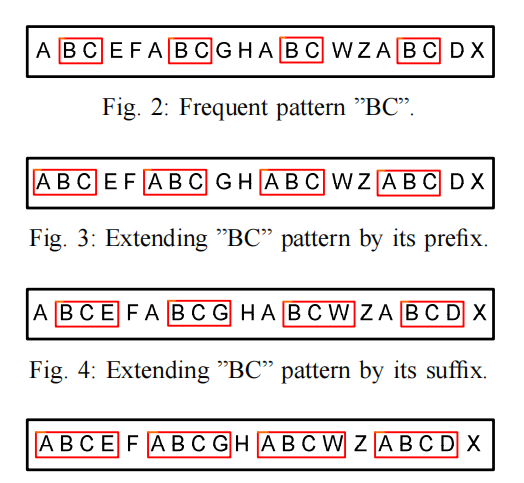
\includegraphics[width=\linewidth]{figures/CASAS}
  \caption{Using Apriori-type algorithm to find rules\cite{rashidi2009keeping}}
\end{figure}
\subsection{Apriori-Based Applications}
The Weka\cite{witten2005practical} implementation of an Apriori-type algorithm is used, which iteratively reduces the 
minimum support until it finds the required number of rules 
within a given minimum confidence. Jakkula\cite{jakkula2007learning, jakkula2007mining} using Weka to identify the frequent 
activities, or events, which occur during the day and establishing temporal relations among them, describes a method of discovering temporal relations 
in smart home datasets and applying them to perform activity prediction on the frequently-occurring events. It tests
various configurations in Weka to find the best rules which can aid the prediction process.

CASAS\cite{rashidi2009keeping} introduce an adaptive smart
home system that utilizes Apriori-Based techniques to discover
patterns in resident’s daily activities and to generate automation
polices that mimic these patterns. Its core algorithm FPAM takes a bottom-up
approach just like Apriori, However, unlike the Apriori algorithm, not only
does it discover frequent sequences, but it also tries to find
periodic sequences and their periodicity. As Figure 1 shows, FPAM extends sequences that made the cutoff in the
previous iteration by the two events that occur before and after
the current sequence instances in the data. FPAM
incrementally increases the window size until no frequent or
periodic sequences within the new window size are found or a
user-defined limit on the window size is reached.

PUBS\cite{aztiria2012discovering} discovers frequent patterns from users’ traces and turns them
into event-driven rules that represent a subset of TAP rules. The ARM algorithm used by PUBS is similar to the
Apriori with only two differences: 1) Limit possible associations with the object under analyzing. 2) The result 
does not consider a pair as a pattern, but only as sensors that can be potentially related in a meaningful way. To implement,
PUBS modify Apriori by adding the aforementioned constraints has been
used in this step. As in every association mining process, minimum coverage, support
and window size values must be provided.
\section{SPADE}
The SPADE (Sequential PAttern Discovery using Equivalence classes) algorithm\cite{zaki2001spade} is the most typical ARM algorithm for \textbf{vertical database}.
vertical organization refers to the representation of objects as columns and with each
row within the dataset representing an item. There are four advantages of the vertical organization over the horizontal
organization\cite{shenoy2000turbo}:
\begin{itemize}
  \item Itemset validation is computationally faster in a vertical layout due to its item focus.
  \item Given the nonmonotonic constraints, items can be easily removed from the dataset, reducing its size.
  \item Vector compression is greater in larger datasets andhence better in a vertical layout as typically the number of objects exceeds the number of items.
  \item Given nonmonotonic constraint inclusion, vertical organization allows the computation of an itemset once its subsets have been deemed
  valid.
\end{itemize}
SPADE use combinatorial properties and lattice-based search techniques, allow constraints to
be placed on the mined sequences. The key features of SPADE include the layout of the database in a vertical id-list
database format with the search space decomposed into sub-lattices that can be processed independently in main memory 
thus enabling the database to be scanned only three times or just once on some preprocessed data.
\begin{figure*}[htbp]
  \centering
  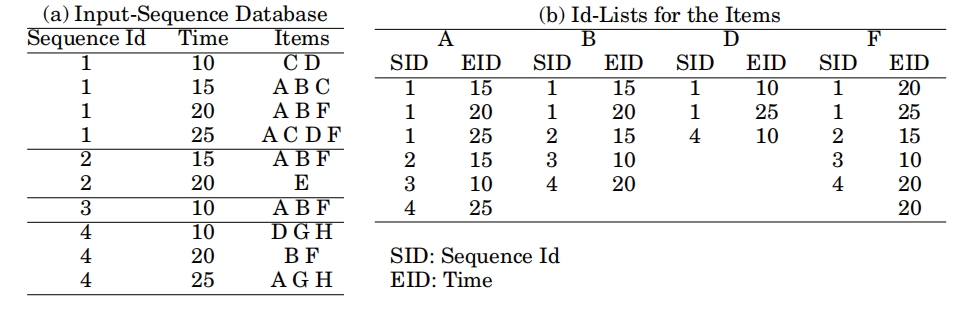
\includegraphics[width=0.85\textwidth]{figures/vertical}
  \caption{Vertical Formatting Data Layout\cite{zaki2001spade}}
\end{figure*}
Using the vertical id-list database in Figure 2, all frequent 1-sequences can be
computed in one database scan. Computing the $F_{2}$ can be achieved in one of two ways:
by preprocessing and collecting all 2-sequences above a user-specified lower bound, or
by performing a vertical to horizontal transformation dynamically.
Once this has been completed the process continues by decomposing the 2-sequences
into prefix-based parent equivalence classes followed by the enumeration of all other
frequent sequences via either breadth-first or depth-first searches within each equivalence class. 
The enumeration of the frequent sequences can be performed by joining
the id-lists in one of three ways:
\begin{itemize}
  \item Itemset and Itemset: joining $AS$ and $BS$ results in a new itemset $ABS$.
  \item Itemset and Sequence: joining $AS$ with $B \to S$ results in a new sequence $B \to AS$.
  \item Sequence and Sequence: joining $A \to S$ with $B \to S$ gives rise to three possible results: a new itemset $AB \to S$, and two new sequences $A \to B \to S$and $B \to A \to S$.
\end{itemize}
\subsection{SPADE-like Algorithm}
The cSPADE algorithm\cite{zaki2000sequence} is the same as SPADE except that it incorporates
one or more of the syntactic constraints as checks during the mining process, including length or width limitations 
on the sequences allows for highly structured data; minimum or maximum gap constraints on consecutive sequence; applying a time window on allowable sequences, requires the entire sequence to
occur within the window; incorporating item constraints.

SPAM (Sequential PAttern Mining using a bitmap representation) \cite{ayres2002sequential} uses a novel depth-first traversal of the search space with various pruning mechanisms
and a vertical bitmap representation of the database, which enables efficient support
counting. A vertical bitmap for each item in the database is constructed while scanning
the database for the first time with each bitmap having a bit corresponding to each
element of the sequence in the database. One potential limiting factor on its usefulness
is its requirement that all of the data fit into main memory.

The CCSM (Cache-based Constrained Sequence Miner) algorithm\cite{orlando2004new} uses a level-wise approach initially but overcomes many problems associated
with this type of algorithm. This is achieved by using k-way intersections of id-lists to compute the support of candidates
When a new sequence is generated, and if a common prefix is contained in the cache, then
the associated id-list is reused and subsequent lines of the cache are rewritten. This enables only a single equality join to be performed between the common prefix and the
new item, after which the result of the join is added to cache.
\subsection{SPADE-base Applications}
EMS (energy management system)\cite{chen2013detecting} provides a non-intrusive and low-cost 
solution to recognize the states of appliances and to disaggregate 
the energy consumption of appliances in a house/building. It use SPADE to detect users' behaviors based on the usage patterns of 
appliances. EMS find that users' behaviors strongly correlate with a 
sequence of appliance usages and appliance states. Therefore, 
it can utilize the data including status of appliance and the 
time that the appliance state changes to detect users' behaviors. user behavior detection is mining 
the sequences from a number of cases. Each case represents an 
activity and its possible correlated events. SPADE algorithm is applied to learn the sequential patterns for each 
activity.

LFE (Load Forecasting Enhancement)\cite{ding2015sequential} gives a set of insights
into household-specific activity sequences influencing power consumption derived from a sequence mining algorithm,
and a load forecasting
study using identified frequent activity sequences as an enhancement.
The implementation utilize the SPADE algorithm to understand a household’s daily activity sequences, a
sequence is given by all the activities performed by the
household throughout a day and ordered by the start time of
activities.

SHGuard\cite{mao2019anomalous} is an anomaly detection approach
based on power usage data exposed from wireless communications in the smart home system.
SHGuard extracts and
builds the normal behavior pattern during the initialization stage. It continuously infers the smart devices’ states
by monitoring the electricity usage data and updates the
user behavior patterns. 
It choose the SPADE algorithm to perform sequential
pattern mining on power-usage behavior sequence dataset, preprocess the
power-usage behaviors dataset and convert it into the standard input data format of the SPADE algorithm, which is
$s = (sequenceID, eventID,item)$, and eventually obtain a frequent sequence pattern set.

\section{PrefixSpan}
PrefixSpan (Prefix-projected Sequential Pattern mining)\cite{han2001prefixspan} is the core algorithm of \textbf{pattern growth algorithm}. The frequent pattern growth paradigm removes the need for the 
candidate generation and prune steps that occur in the Apriori-type algorithms and does so by compressing the database representing the 
frequent sequences into a frequent pattern tree and
then dividing this tree into a set of projected databases, which are mined separately\cite{han2000mining}.

PrefixSpan use \emph{projected databases}, A subsequence
$\alpha'$ of sequence $\alpha$ is called a projection of $\alpha$ with respect to prefix $\beta$ if and only
if 1) $\alpha'$ has prefix $\beta$, and 2) there exists no proper supersequence $\alpha''$ of $\alpha'$ such that
$\alpha''$ is a subsequence of $\alpha'$ and also has prefix $\beta$. PrefixSpan works based
on recursively constructing the patterns by growing on the prefix, and simultaneously,
restricting the search to projected databases. This way, the search space is reduced at
each step, allowing for better performance in the presence of small support thresholds.

The major benefit of this approach is that no candidate sequences need to be generated or tested that do not exist in a projected database. That is, PrefixSpan only
grows longer sequential patterns from shorter frequent ones, thus making the search
space smaller. This results in the major cost being the construction of the projected
databases, which can be alleviated by two optimizations. The first, by using a bilevel
projection method to reduce the size and number of the projected databases, and second
a pseudo-projection method to reduce the cost when a projected database can be wholly
contained in main memory.


Modern big data processing frameworks, including Hadoop, Spark\cite{zaharia2010spark} and
Flink\cite{carbone2015apache}, were all implemented in object-oriented languages such as Scala and Java, due to 
theirs applicability across heterogeneous distributed clusters, convenience on memory management, and fertility 
of community resources. However, big data applications suffer from striking high GC cost under JVM. As reported by users and researchers,
GC time can take even more than 50$\%$ of the overall application execution time in some cases\cite{stackoverflow, bu2013bloat}.
Some concurrent GC algorithms, e.g., G1 GC\cite{detlefs2004garbage}, are able to limit GC pause times to a certain extent, 
while mutator threads would be inevitably affected\cite{xu2019experimental, wu2020platinum}.

The GC inefficiency problem under big data processing frameworks has been widely studied\cite{xu2019experimental,bruno2018study,gidra2013study}, 
and results from a combination of factors. First, big data applications are both \emph{data-intensive} and \emph{memory-intensive}, a large amount of data 
is loaded in the memory as objects at the runtime, putting servere overhead on the GC colloctor. Big data processing frameworks that caching intermediate 
computing results in the memory make thins even worse.
 Second, the memory usage pattern of big data applications is totally different from traditional Java applications, data objects of big data applications tend to stay in memory
 for a long period of time, which is opposite to the\emph{weak generational hypothesis hypothesis}\cite{weakgenerational} that the classical GC algorithms based on.
 
The weak generational hypothesis states that most objects survive for a short time and only a few objects live long. For this reason, popular GC colloctors
are implemented generational, i.e., divide the heap into generations, typically young generation for keeping short-lived objects, and old
generation for keeping long-lived objects. Thus by collecting the young generation more frequently than old generation, GC colloctors reduce the average number of objects 
processed per GC cycle. 

Under generational GC algorithms, long-lived data obejcts are destined to survive in \emph{minor GC} cycles, which is target at young generation,
and certain to be promoted to the old generation eventually when their survival times reach a certain threshold. In each GC cycle, all the long-lived data obejcts would be marked
as "live" objects by the \emph{accessibility analysis} across the object reference graph, and be compacted (copied) to another memory space. Even after being promoted, these
long-lived obejcts would still not be "dead" in a short time, while their big volume makes it very likely to trigger \emph{major GC} when the old generation is full, 
which introduces more unnecessary scan and copy of them. 
As objects marking and moving are considered to be the most time-consuming part of the GC cycle\cite{suo2018characterizing,yu2016performance}, the long-lived data objects is regarded
as the main reason to the degradation of GC efficiency and the main direction of optimization.

Moving back to unmanaged languages and leave memory management to developers is a tiring but possible solution\cite{chenSM,maas2017return}. However, unmanaged languages are error-prone,
espicially to big data applications whose memory usgae is stressful and complicated and whose running time is quite long. Furthermore, since a great number of existing
big data processing frameworks are already developed in a managed language, it is unrealistic to re-implement once again\cite{nguyen2015facade,bruno2018study}. Some other works
 attempt to use the APIs from package \emph{sun.misc.Unsafe} to handle the off-heap memory explicitly like unmanaged languages\cite{mastrangelo2015use,navasca2019gerenuk,nguyen2015facade}.
 The problem is that, as the warning of its name, \emph{Unsafe} package is unsafe. It has the drawbacks same as unmanaged languages, and it may introduce serialization/deserialization
 jobs in orginal big data environment. Therefore, more works still settle the long-lived objects in heap.Two main optimization techniques used in these work are lifetime-based 
 memory management and region-based memory management. The former obtains the lifetime of data objects by static analysis of source code and users' annotation, reclaim the 
 long-lived objects at their "dead" point in the code. The latter leverages the lifetime information to divide the data obejcts by their live time into separate memory spaces, 
 facilitates one-time reclamation\cite{lu2016lifetime,kolokasis2020say,nguyen2016yak,cohen2015data,wang2019panthera}. 
 
Inspired by the techniques above, we pick out the long-lived objects according to the lifetime information, and pretenure them in the older generation. As G1 GC are naturely region-based,
we directly create a new generation aiming at the storage of long-lived data objects on the top of G1, whose regions would neither be involved in minor GC, nor be in the collection sets of major GC, unless it get the signal that the lifetime of the objects in current region is end. 
Thanks to Spark Tungsten\cite{Tungsten} project and Flink who utlizing primitive arraies as memory
pages to form unmanaged-languages-like condition on heap, we could readily pretune most long-lived data by pretuning memory page objects(primitive arraies). We evalute our idea 
by the time costed to creat memory pages. Result shows that, compared with orginal G1 GC, we eliminated 90$\%$ of minor GC pause time.

\section{Motivation}
The main challenge of pretenuring in JVM is determining the long-lived objects. Previous pretenuring works using sampling\cite{harris2000dynamic,jump2004dynamic}, profiling\cite{blackburn2001pretenuring,bruno2019runtime,bruno2017polm2} 
and annotation\cite{bruno2017ng2c} to speculate the lifetime of all the objects. These approches inevitably introduce repeat executions, CPU competition or heavy users' efforts, many of works are highly dependent on the users' developement experience
and knowledge on GC algorithm. Fortunately, long-lived objects determination is simpler under big data processing framworks for the characteristics below:

\subsection{Data Path}

More than 95$\%$ of runtime objects are created and used by a rather small and simple code referred as \emph{data path}, that primarily conducts data manipulation like map, 
reduce, and relational operations. The objects created by \emph{data path} are \emph{data objects}, which are the main component of a long-lived objects. Only less than 5$\%$
 of runtime objects are created by a large and complex code referred as \emph{control path}.The \emph{control objects} created by \emph{control path} are principally 
 for cluster management, scheduling, communication, and others, which are basiclly short-lived and negligible\cite{nguyen2015facade,navasca2019gerenuk,bu2013bloat,nguyen2016yak}. This insight
 allow us focus on a small amount of code when handling long-lived data objects in big data applications, rather than pay attention to massive code in ordinary Java applications.

\subsection{Memory Pages}

As storing the data as objects requires additional memory footprint, some works use primitive array as memory pages to store the data value only. 
The structure of a data object in the JVM contains object headers and references to other objects, and the data value itself usually takes up no more than half of the space 
in the object\cite{navasca2019gerenuk,bu2013bloat}. For the reason that the methods of the data object are seldom used, the "shells" of objects is not only meaningless, but also harmful as it 
introduces serialization/deserialization work when the data is transformed across the cluster through the network, which may accounte for 30$\%$ of the total execution time\cite{navasca2019gerenuk,nguyen2018skyway}   
Therefore, these works allocate primitive array as memory page or memory container, gather the data with similar lifetime in the same memory page, and manage the long-lived data 
as a whole by managing the memory page objects\cite{navasca2019gerenuk,bu2013bloat,nguyen2015facade,lu2016lifetime}, reclaim the memory pages at the end of iterations, stages and
computing operators.

\begin{figure*}
  \centering
  \subfigure[Memory Block of Spark]{
    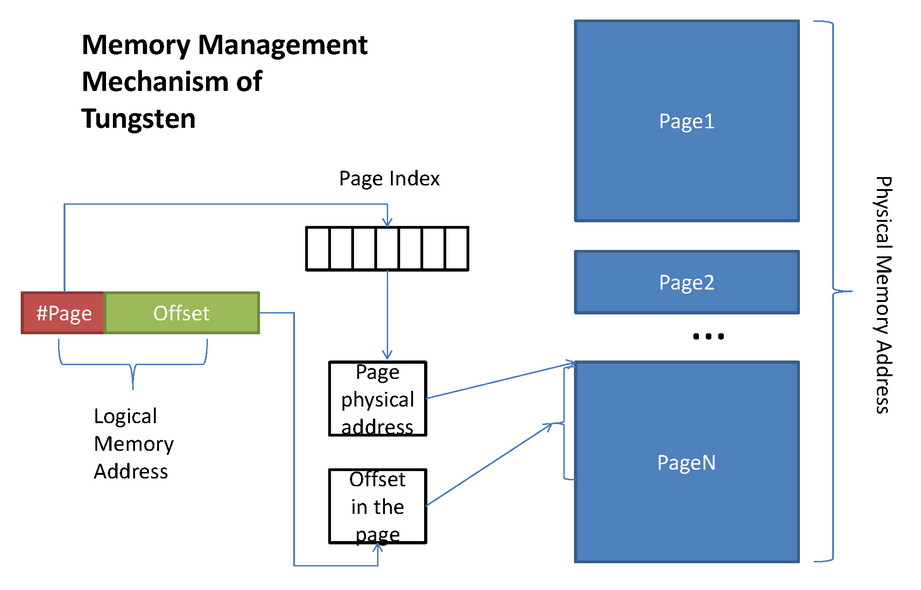
\includegraphics[width=0.45\textwidth]{figures/memoryblock}
  } 
  \subfigure[Memory Segment of Flink]{
    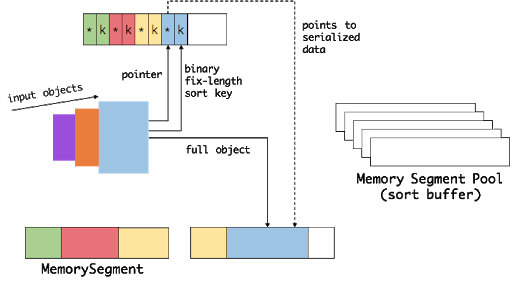
\includegraphics[width=0.45\textwidth]{figures/memorysegement}
  } 
  \caption{Memory Page in Modern Big Data Processing Framworks.}
\end{figure*}

Modern big data processing framworks utilized the idea of memory page, store the serialized data value in the memory page. As shown in Figure 1(a), Tungsten project of Spark uniform the in-heap and off-heap memory by memory blocks,
Tungsten manages memory blocks as page table. The memory location of a data value is determined by the page number and the offset in page. Off-heap page number is represented by an 
absolute address, and the page offset is the current address. On-heap page number is represented by the reference to the corresponding array object, and the offset in page 
is the relative offset within the array object. When the data in the page are freed explicitly by Spark, the memory page object would be added to a memory pool made up by weak reference, 
which means the memory page either be reused before it is scanned, or be relcaimed in next GC cycle. 

Similar to Spark Tungsten, Flink serializes objects into a fixed number of memory segments. As shown in Figure 1(b), memory manager of Flink holds a huge collection of 
memory segments in the memory pool. Different from memory blocks of Spark, memory segment is pre-allocated and fixed-sized, whose default size is 32KB. In addition, the lifetime of memory segments in the memory pool is 
same as computing task, it would only be released when the task end.

Design of memory page brings remarkable performance improvement to the big data processing frameworks, the reasons are as follows. (1) The binary form of data in memory page increases the storage density of memory, which allows more data cached
in the memory. The employment of memory page decreases the number of objects, i.e., reduces the pressure of GC. (2) The frameworks implements specialized serializer and computing
operators aiming at binary data speed up the execution and data transmission. (3) The continuous arrangement of data in memory page improves the spatial locality of memory accessment, 
 which is a great concern of current GC algorithm for it improves L1/L2/L3 cache hit ratio of CPU\cite{yang2020improving,li2019scissorgc}. 
 
 The contradiction is the choice between on-heap and off-heap, which are both available in Flink and Spark. The benefits of using off-heap are attractive, nevertheless the usage of off-heap is not safe and secure under big data frameworks as discussed in section 1, and Java Unsafe package is not available since JDK 11\cite{UnsafeRemove}. 
 Therefore, allocating memory pages on heap is the most likely direction for the future. The left problem is, the cost of promoting memory pages and major GC is still noteworthy
 in a large memory environment\cite{MinorGCLong}, which can be solved exactly by pretenuring. The clear type and size of memory page makes this work achievable.

\section{Desgin and Implementation}
  We implement our idea in the OpenJDK 8 HotSpot JVM, one of the most widely used industrial JVMs. Since HotSpot is a highly optimized production JVM, our algorithms were implemented carefully
to prevent the other function and the overall performance of JVM, some analysis and choices are made during the implementation procedure. Essential details are as follows.

\subsection{Pick Out Long-Lived Objects}
  Cached records and accumulated shuffled records are the main source of long-lived data objects in big data processing framworks\cite{xu2019experimental}. Cached records stand for
reusable data which are retained in memory by developers, in order to reduce disk I/O. Developer explicitly caching data using method \emph{cache()} or \emph{persist()}, and release them 
from memory using method \emph{unpersist()}. Cached \emph{Resilient Distributed Dataset} (RDD) in Spark is a typical example that we focus on. The lifetime of shuffled records
is more complicated, nevertheless, they are handled in memory pages. Therefore, we can only focus on memory block and memory segment.

As discussed in section 2.1, the manipulation of data objects is accomplished by a few code in data path. There is no exception on cached RDD, memory block and memory segement.
The building function of these three kinds of objects are respectively:  
\begin{itemize}
  \item \textbf{Memory segement}: \emph{byte} type array of fixed size 32K;
  \item \textbf{Memory block}: \emph{long} type array of required data size;
  \item \textbf{Cached RDD}: Array of user-defined type with required length, each element is of user-defined type.
\end{itemize}

The next job is letting JVM figure out thses long-lived objects at runtime. Dispose of memory segement and memory block is rather straightforward, as they are primitive types array, 
the creation of them are done by corresponding initialed \emph{TypeArrayKlass} in JVM, respectively \emph{byteArrayKlassObj} and \emph{longArrayKlassObj}. For the memory segement 
is fixed-sized, we identify it by the size when allocating. Though the length of memory block varies, it is generally longer than the length of ordinary long type array, we identify a long type array memory
block if its length exceeds a threshold, the rest memory blocks whose length smaller than threshold are rather negligible. Dispose of cached RDD is rather difficult, for the element object of cached RDD may contain 
variety types of objects, we only handle the RDD array. Even so, we still can not identify it without the help from code of big data processing frameworks. We pass the user-defined type \emph{T}
 to the JVM, and identify \emph{T} type array cached RDD if its length exceeds threshold, which is a common approch to identify RDD array\cite{wang2019panthera}.         

\subsection{GC Colloctor Choice}
After figured in the JVM, the allocation request of long-lived object is passed to the allocator, which varies from GC algorithm. There are two reasonable choice: 
Parallel scavenge GC and G1 GC, two most widely used GC collectors in HotSpot. Parallel is the default collector of JDK 8, which is the most popular version of JDK. 
G1 is the default collector since JDK 9, and is explicitly set as the default collector in Flink.

As shown in Figure 2, the distinct difference between Parallel and G1 is that, the young and old generations are both contiguous space with an explicit boundary in Parallel, and major GC would handle the whole heap space, while G1 logically separates young and old generations in a non-contiguous way, by dividing
heap space into a large number of equal-sized regions, each region can be young or old space, only some garbage-filled heap regions picked in the collection
 set would be handled during most major GC. Specially, Parallel store humongous objects directly into old generation, and G1 stores humongous objects 
 into humongous regions, which span multiple regions in old generation.
\begin{figure}[h]
  \centering
  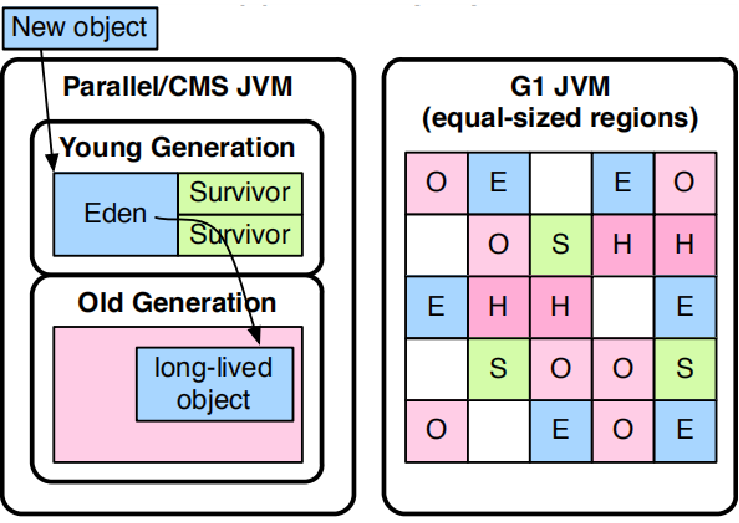
\includegraphics[width=\linewidth]{figures/GCalgorithm}
  \caption{Heap distribution under Parallel scavenge GC and G1 GC algorithm}
\end{figure}
Pretuning is easy to implement in Parallel GC, as the method of humongous objects allocation is relatively exposed, using this method could directly settle the
long-lived memory pages in the old generation without the modification of heap lock in JVM. However, memory pages pretuned in Parallel are mixed with other
ordinary objects promoted in old generation, still need to be scanned and moved during major GC, for major GC of Parallel target at whole heap space. Also the 
locality of memory pages may be damaged by compact phase of major GC, since the compact job is done by multiple GC threads, the new order of memory pages is uncertain.
which makes the memory access sequence unfriendly to data sequence, degrades the L1/L2/L3 cache hit ratio of CPU. Besides, evaluation of garbage collectors on big
data applications shows that Parallel always introduce long pause time and tail latency\cite{xu2019experimental,suo2018characterizing,yu2016performance,li2019scissorgc},
much inferior to G1 GC. For these reasons, Parallel is not our preference choice. 

Modify on G1 GC could avoid the problems above. As G1 divides the heap space into regions, we use some of these regions to store long-lived memory pages to seperate 
them from ordinary objects and protect the locality of memory pages. To address unnecessary scan and movement during major GC, we let the regions that store
memory pages skip away from collection set of G1 GC unless JVM get the release signal from big data processing frameworks. During major GC, G1 would only handle the 
regions in the collection set, thus memory pages would not be moved. In addition, memory page have no reference to other objects for the reason that it is only a 
carrier of data, which reduces the overhead of scan and footprint of remember set, which record the reference across the regions in G1 GC. 

In implementation, we name these regions 
\emph{Keep} regions in JVM, distinguish them from the normal old regions. Memory space occupied by \emph{Keep} regions still count in old generation space, 
in order to keep the overall memory apportion of young and old generation.   

\subsection{Memory Allocation Buffer}
Using humongous objects allocation method in G1 GC to allocate long-lived memory pages is unbearable. Because every humongous object allocation would occupy
at least one heap region, whose size is much bigger than a memory page object. More importantly, humongous object allocation is in the slow path of objects allocation, i.e., 
required memory is obtained by heap lock competition, which is inefficient.

Allocation memory competition between different threads is solved by Thread Local Allocation Buffer (TLAB) in young generation and Promotion Local Allocation Buffer (PLAB)
in old generation. As the example of TLAB in Figure 3, JVM divides the free memory space into allocation buffers, each buffer dedicated to a particular thread. 
since every thread allocate objects in the allocation buffer belong to it, there is no need for synchronization. 
Though we count keep regions in old generation, while PLAB is only used during GC for GC thread, we use TLAB in keep
regions for mumator thread. For mumator thread already have a TLAB for young generation, we add another TLAB for keep regions and change the way mutator thread
get TLAB, using pointer instead of offset to the base address of thread.

The size of TLAB is initialed when JVM start on the basis of the total heap size, and update at the end of each GC cycle according to the  \emph{Adaptive Policy}.
Since memory page is larger than ordinary object, while TLAB size update is globally, we adjust the size of TLAB for keep regions independently. As the size of
memory page is known, we set this size to a reasonable value, which can reduce TLAB waste, increases the number of memory pages a TLAB could continuously allocate 
without heap lock, consequently reduce the TLAB allocation throguh slow allocation path. 

\begin{figure}[h]
  \centering
  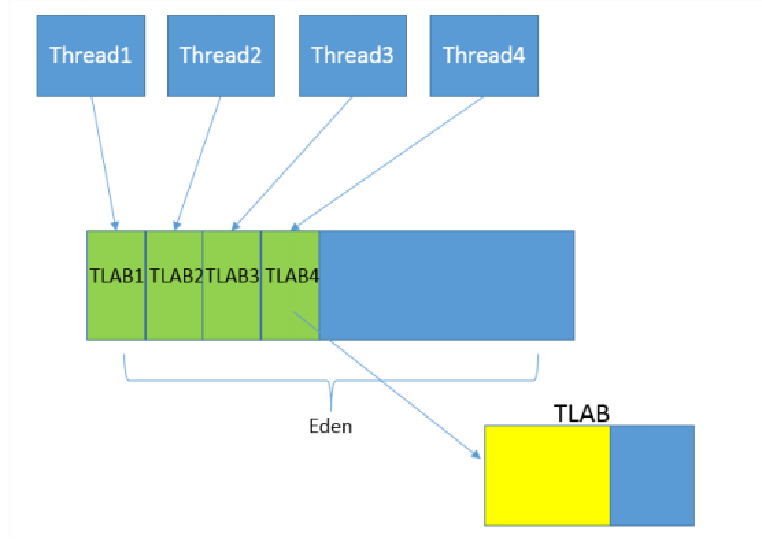
\includegraphics[width=\linewidth]{figures/TLAB}
  \caption{Thread Local Allocation Buffer}
\end{figure}

\section{Evaluation}
We evaluate our desgin by allocating memory pages, and we use representative big data processing frameworks Flink to verify the feasibility of our implementation.
The result shows that, compared with orginal G1 GC, our implementation could achieve shorter execution time and GC pause time, less object movement and remember set
footprint without negative effect on other functions.

\subsection{Evaluation Setup}

\subsection{TLAB Size}

\subsection{GC Pause Time}


%%
%% The next two lines define the bibliography style to be used, and
%% the bibliography file.
\bibliographystyle{ACM-Reference-Format}
\bibliography{mybib}

\end{document}
\endinput